
\chapter {Introducción}
\label{sec:intro}


    El acceso a la vivienda compartida define la rutina de miles de universitarios y jóvenes profesionales en toda España. La escalada de precios del alquiler en las ciudades universitarias transformó una experiencia temporal de dos cursos en un régimen residencial obligado que se prolonga durante años. Alquilar una habitación ya no es una elección casual. Supone la única alternativa económica viable ante el encarecimiento desmedido de los inmuebles completos.

    Los programas de intercambio internacional intensifican este problema. Cada semestre llegan estudiantes bajo convenios Erasmus que se ven forzados a reservar habitación a ciegas desde el extranjero, sin visitar el piso físico y negociando en idiomas que apenas dominan. Fiarse de fotografías sueltas en anuncios dudosos genera incertidumbre real. El riesgo económico resulta patente.

    La dispersión de canales agrava estas dificultades iniciales. La mayoría de arrendamientos entre particulares se siguen tramitando mediante grupos informales en redes sociales, anuncios clasificados genéricos o acuerdos verbales sin respaldo. Esta falta de estructura acarrea abusos contractuales, pérdida de depósitos y un cruce caótico de mensajes entre las partes antes de cerrar cualquier trato.

    Las fricciones continúan una vez dentro de la vivienda. Entrar al piso abre un segundo frente organizativo: quién limpia las zonas comunes, cómo se liquidan las facturas de suministros y qué normas rigen los espacios compartidos. Resolver estas responsabilidades con notas adhesivas o hilos caóticos de mensajería fracasa sistemáticamente. Se generan malentendidos y desequilibrios en el reparto doméstico que desgastan la convivencia diaria.

    
\section{Justificación}
\label{sec:justificacion}

    El desarrollo de Colivi surge de una necesidad práctica vivida en primera persona durante estancias de intercambio universitario. Buscar habitación a cientos de kilómetros revela un mercado opaco. Los anuncios omiten detalles esenciales, los arrendadores tardan días en contestar y las condiciones económicas varían sobre la marcha sin dejar constancia escrita. El estudiante asume un desembolso económico sin garantías reales sobre el estado del piso ni la identidad de quien cobra la fianza.

    La convivencia posterior destapa nuevos roces cotidianos. Una vez formalizada la estancia, el grupo debe coordinar turnos de limpieza, compras compartidas y pagos de suministros. Confiar este control a pizarras domésticas o chats grupales suele terminar en disputas. La ausencia de un registro inmutable dificulta comprobar quién ha cumplido sus obligaciones y quién acumula retrasos continuados en los gastos.

    Las aplicaciones comerciales resuelven únicamente fragmentos aislados de este ciclo. Existen portales inmobiliarios centrados en captar inquilinos y aplicaciones móviles diseñadas para anotar gastos entre amigos, pero ninguna herramienta enlaza la reserva formal con la vida diaria dentro de la vivienda. Colivi conecta ambos momentos bajo un mismo sistema. La plataforma combina un backend en Spring Boot 3 con tipado estricto, una interfaz reactiva construida en React y un servidor auxiliar bajo el protocolo MCP (\emph{Model Context Protocol}) para consultar datos mediante modelos de lenguaje, cerrando la brecha entre la búsqueda inicial y el régimen diario del piso.


\section{Objetivos Y Estructura}
\label{Objetivos Y Estructura}

    Diseñar y construir Colivi constituye el objetivo principal de este proyecto, ofreciendo una plataforma web que da respuesta a la búsqueda de habitaciones y a la organización interna en pisos de estudiantes. La aplicación acompaña a los usuarios durante todo el ciclo: conecta al arrendatario con el propietario durante la reserva y estructura el reparto de tareas domésticas una vez comenzada la convivencia.
    
    La consecución de esta meta global se desglosa en los siguientes objetivos específicos:

\begin{enumerate}
    \item Implementar un módulo de seguridad para registro e inicio de sesión mediante tókenes JWT, distinguiendo perfiles de inquilino y propietario.
    \item Habilitar la edición del perfil de usuario con datos de contacto, preferencias y hábitos de convivencia.
    \item Desarrollar un buscador de habitaciones con filtrado por localización geográfica, precio mensual, equipamiento y normas de estancia.
    \item Construir un canal de mensajería contextual asociado a cada anuncio que permita plantear dudas al anfitrión sin exigir una reserva previa.
    \item Programar el ciclo de vida de las solicitudes de reserva con control estricto de estados y depósitos de fianza.
    \item Diseñar un planificador gamificado de tareas domésticas basado en turnos rotativos (\emph{Round-Robin}), tabla de puntuaciones y posibilidad de rescate entre compañeros.
    \item Disponer un registro inmutable de auditoría para monitorizar acciones clave dentro del hogar, como la realización de limpiezas o la incorporación de nuevos miembros.
    \item Integrar un asistente inteligente fundamentado en el protocolo \emph{Model Context Protocol} (MCP) que consulte turnos, resuma actividad o filtre anuncios sin modificar la base de datos.
\end{enumerate}

    La arquitectura global del sistema (reflejada en la figura~\ref{fig:estructura_tecnica_colivi}) distribuye sus responsabilidades en cuatro capas desacopladas: el cliente web, el servidor central de aplicaciones, el microservicio de soporte inteligente y el motor de persistencia relacional.

    El cliente web interactúa directamente con el usuario mediante una interfaz reactiva construida con React, TypeScript y Tailwind CSS. Vite actúa como empaquetador para optimizar los tiempos de recarga durante el desarrollo y minimizar el tamaño del paquete final en producción. La sincronización de datos asíncronos recae en TanStack Query, aplicando una estrategia de sondeo controlado (\emph{Smart Polling}) que refresca los mensajes y las tareas únicamente mientras la pestaña del navegador permanece en primer plano, evitando la sobrecarga de conexiones persistentes innecesarias.

    El backend principal se ejecuta sobre la máquina virtual de Java 21 utilizando Spring Boot 3. Este servidor expone una API REST dividida en módulos de dominio bajo principios SOLID. Procesa reglas de negocio críticas: el reparto equitativo de turnos de limpieza, la desvinculación automática de reservas mediante eventos internos de dominio (@EventListener) y la contención de colisiones concurrentes mediante bloqueos pesimistas en las tablas afectadas. Asimismo, se apoya en Spring AI para consultar modelos de lenguaje remotos a través de la API de Groq, devolviendo respuestas formateadas en JSON estricto.

    Un microservicio complementario desarrollado en Node.js y TypeScript expone un servidor MCP oficial mediante \emph{Server-Sent Events} (SSE). Este servicio declara herramientas de inspección de anuncios, consulta de estado de tareas y cola de moderación. Cada conexión hereda el token JWT emitido por el backend, imponiendo un aislamiento estricto de solo lectura para evitar que la inteligencia artificial altere tablas de forma directa.

    La persistencia de datos reside en un clúster relacional de PostgreSQL. Mediante JPA e Hibernate se gestionan las entidades de usuarios, publicaciones, conversaciones, trazas de auditoría y turnos periódicos. Se aplicaron índices compuestos y restricciones de unicidad para descartar registros duplicados y mantener la integridad referencial en todo momento.

\begin{figure}[htbp]
    \centering
    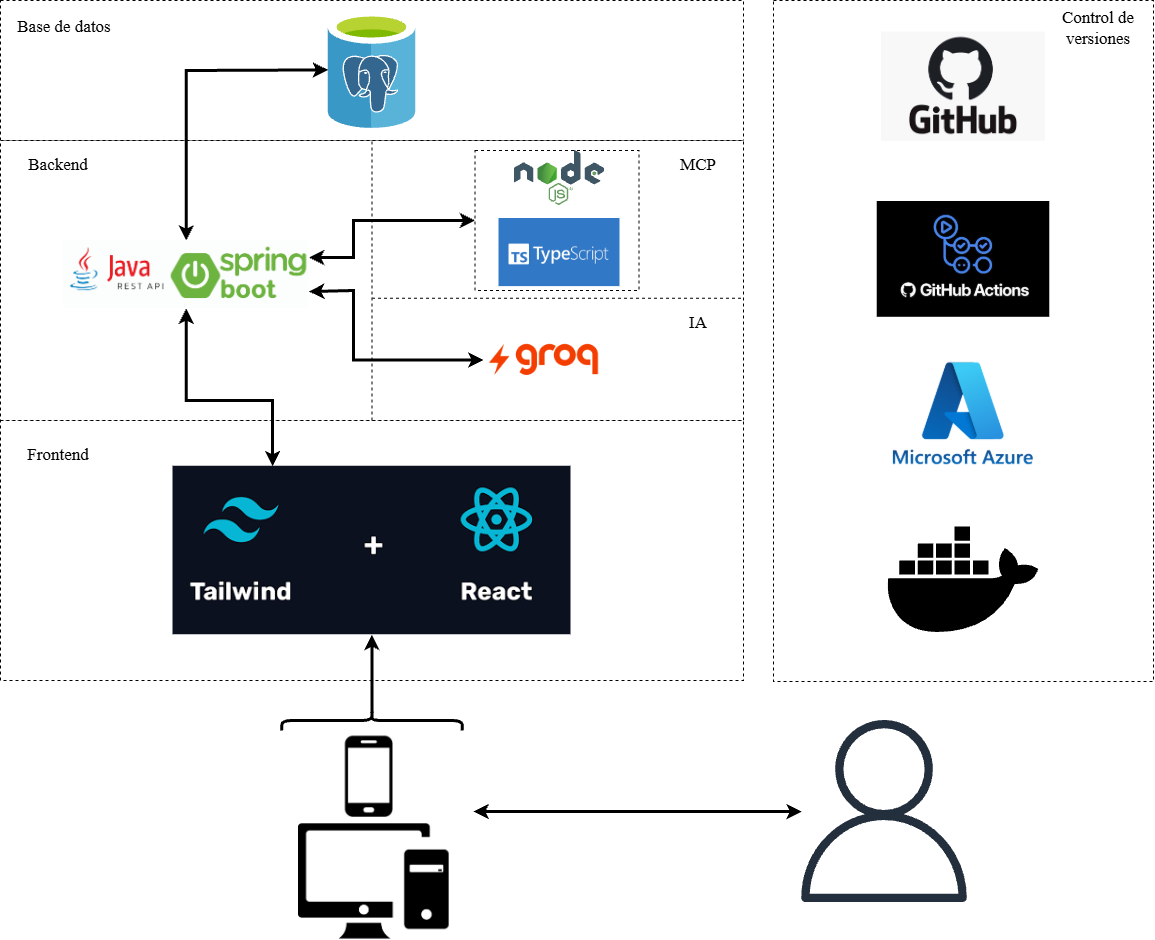
\includegraphics[width=0.85\textwidth]{Introduccion/img/Figura1.1.png}
    \caption{Estructura técnica global y arquitectura de la plataforma Colivi}
    \label{fig:estructura_tecnica_colivi}
\end{figure}

\section{Planificacion}
\label{Planificacion}

    El proyecto abarca una carga docente estipulada de 12 ECTS, equivalente a 300 horas de dedicación en el plan de estudios del Grado en Informática. El cronograma cubre la toma inicial de requisitos, el modelado del dominio, la codificación del sistema distribuido, la integración de modelos de lenguaje y la redacción de la memoria. La figura~\ref{fig:planificacion_temporal_general} recoge la descomposición temporal de este trabajo.

    El trabajo preliminar absorbió 100 horas repartidas durante el primer mes: evaluación tecnológica (30 horas), especificación de requisitos del sistema (30 horas) y diseño de maquetas de interfaz (40 horas). Esta fase sirvió para contrastar la viabilidad del protocolo MCP con Spring AI, verificar la velocidad de inferencia del proveedor Groq, normalizar las tablas en PostgreSQL y cerrar los flujos de navegación antes de codificar la solución.

    El núcleo de programación concentró 170 horas de esfuerzo. La construcción de la aplicación web y los microservicios acaparó 110 horas, programando la lógica de negocio en Spring Boot 3, el cliente web en React con TanStack Query y el servidor MCP en Node.js. Sobre esta base funcional se desarrollaron tres hitos derivados: el empaquetado móvil sobre Android con Capacitor (25 horas), la definición de contenedores Docker y el despliegue en la nube de Microsoft Azure (20 horas), y una batería final de pruebas de integración con JUnit y Mockito (15 horas) para verificar la consistencia transaccional y la autenticación sin estado.

    Las 30 horas finales se asignaron a redactar la memoria en LaTeX conforme a las pautas tipográficas de la Escuela Superior de Ingeniería, generar los diagramas formales en PlantUML y preparar la defensa ante el tribunal. La redacción se abordó con el software ya estabilizado, garantizando que el texto reflejara el comportamiento exacto de las rutas, entidades y eventos implementados.

\begin{figure}[htbp]
    \centering
    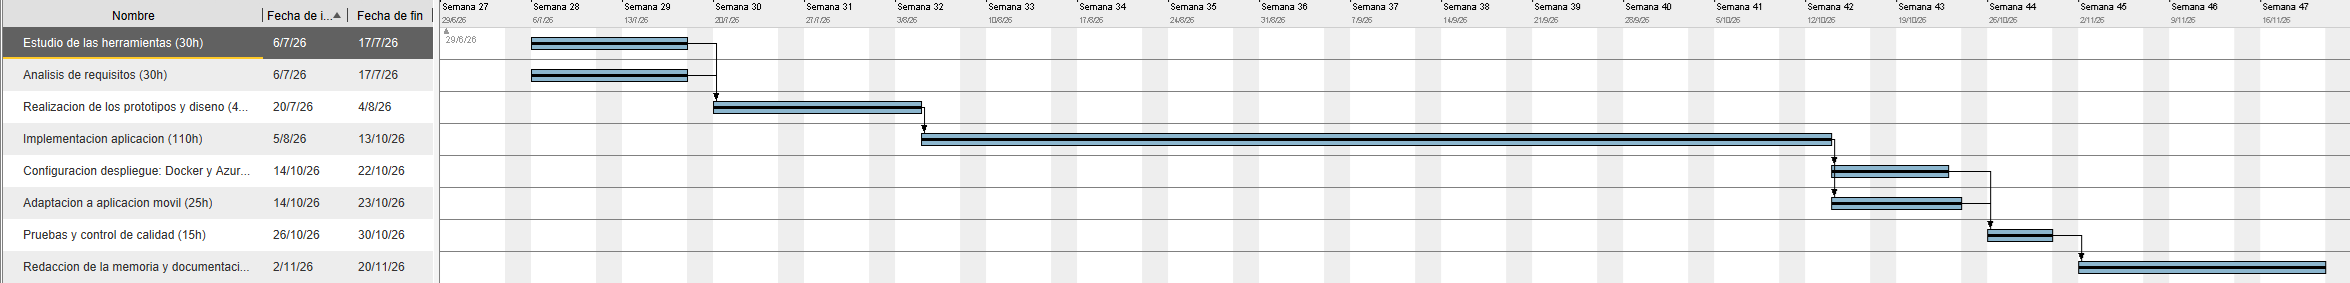
\includegraphics[width=0.85\textwidth]{Introduccion/img/Planificacion.png}
    \caption{Planificación Temporal General}
    \label{fig:planificacion_temporal_general}
\end{figure}

    Las 110 horas dedicadas al desarrollo exigieron planificar qué módulos podían ejecutarse en paralelo y cuáles imponían una secuencia obligatoria por dependencias de datos.

    El trabajo simultáneo aceleró las capas base: mientras se levantaban las entidades JPA y las migraciones en PostgreSQL, se maquetaba el armazón de rutas y componentes en React con Tailwind CSS. La autenticación local mediante tókenes JWT y el inicio de sesión federado con Google OAuth se construyeron en paralelo a sus formularios web en el cliente. De igual manera, el buscador de alojamientos avanzó al mismo tiempo que el mapa interactivo de Leaflet, pues ambas vistas consumían los mismos endpoints REST del backend.

    Las reglas de negocio troncales requirieron un avance estrictamente secuencial debido a restricciones del modelo relacional:

\begin{enumerate}
    \item \textbf{Gestión de alojamientos y catálogo}: habilitó la persistencia de propiedades, la subida de fotografías a Cloudinary y la definición de comodidades antes de admitir cualquier interacción.
    \item \textbf{Solicitudes de reserva y cobro de fianza}: se apoyó en el catálogo activo para gestionar rangos de fechas sin colisiones temporales y conciliar el abono de la fianza.
    \item \textbf{Espacio del hogar}: se instanció como contenedor lógico derivado de una reserva confirmada y abonada, agrupando a los inquilinos aceptados.
    \item \textbf{Gastos compartidos y tareas domésticas}: dependían de la existencia previa del hogar. Se implementó el motor de saldos contables con simplificación de deudas y, tras verificarlo, se programó el reparto rotativo de limpieza con asignaciones periódicas y recompensas.
    \item \textbf{Mensajería contextual}: se construyó sobre la convivencia constituida, permitiendo conversaciones entre compañeros de piso o entre inquilinos y propietarios.
    \item \textbf{Asistente virtual (Spring AI y MCP)}: se integró tras estabilizar los endpoints de catálogo y tareas, permitiendo que el servidor MCP consumiera datos consolidados sin lidiar con contratos cambiantes en la API interna.
    \item \textbf{Moderación, valoraciones y RGPD}: cerró el sistema antes de la fase de despliegue, añadiendo denuncias disciplinarias, reseñas mutuas y políticas de supresión de datos personales.
\end{enumerate}

\begin{figure}[htbp]
    \centering
    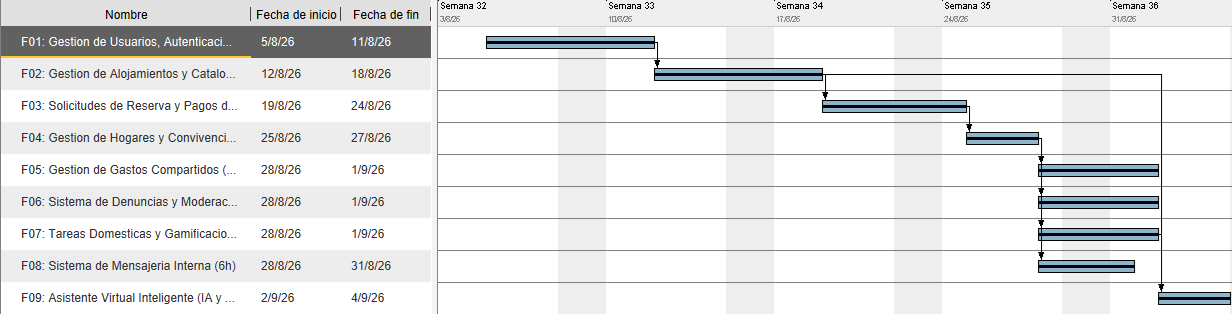
\includegraphics[width=0.85\textwidth]{Introduccion/img/planificacionImplementacion.png}
    \caption{Planificación Temporal de la implementación}
    \label{fig:planificacion_temporal_implementacion}
\end{figure}

\section{Apps Similares}
\label{sec:Apps Similares}

    Examinar el mercado de software actual permitió delimitar los patrones de diseño consolidados y constatar qué carencias sufren los usuarios en su día a día. Existen herramientas consolidadas para cada fase por separado, pero ninguna cubre el recorrido completo. Se seleccionaron cinco plataformas representativas: portales de captación inmobiliaria generalista como Idealista~\cite{idealista}, servicios de alojamiento temporal como Airbnb~\cite{airbnb}, redes de alquiler por habitaciones como Badi~\cite{badi}, gestores contables como Tricount~\cite{tricount} y organizadores de tareas domésticas como Flatastic~\cite{flatastic}.

    Idealista~\cite{idealista} (figura~\ref{subfig:idealista}) domina el mercado inmobiliario en España gracias a su catálogo masivo y a un motor de búsqueda geográfica ágil. Su modelo de negocio se limita a la intermediación publicitaria inicial. El portal se desentiende por completo una vez establecido el contacto entre anunciante e interesado: no custodia fianzas, no verifica identidades mediante contratos formales y carece de herramientas para organizar la vida comunitaria tras la entrega de llaves.

    Airbnb~\cite{airbnb} (figura~\ref{subfig:airbnb}) dispone de una pasarela de pagos consolidada, gestión de depósitos en garantía y verificación de identidades mediante valoraciones recíprocas. Sin embargo, su orientación es turística. Las comisiones por servicio resultan prohibitivas para alquileres residenciales de media y larga duración. Tampoco contempla dinámicas de convivencia entre compañeros que comparten un mismo piso durante meses, delegando cualquier acuerdo interno a la comunicación informal externa.

    Badi~\cite{badi} (figura~\ref{subfig:badi}) nació orientada al alquiler de habitaciones en grandes núcleos urbanos, filtrando cuartos libres y perfiles de candidatos mediante un chat integrado. Pese a coincidir con la fase de captación de Colivi, su utilidad concluye con el acuerdo de entrada. La aplicación no acompaña a los inquilinos en el día a día: queda fuera cualquier herramienta para auditar gastos compartidos, coordinar la limpieza o dirimir desacuerdos domésticos.

    Tricount~\cite{tricount} (figura~\ref{subfig:tricount}) resuelve con solvencia el reparto de gastos mediante la simplificación de grafos de deuda entre múltiples participantes. Funciona como una libreta contable aislada. Carece de contexto inmobiliario real: los compañeros deben introducir cada concepto a mano sin vincularlo a contratos de alquiler, recibos oficiales o depósitos de fianza gestionados de forma conjunta con el propietario.

\begin{figure}[htbp]
    \centering
    \begin{subfigure}[b]{0.49\textwidth}
        \centering
        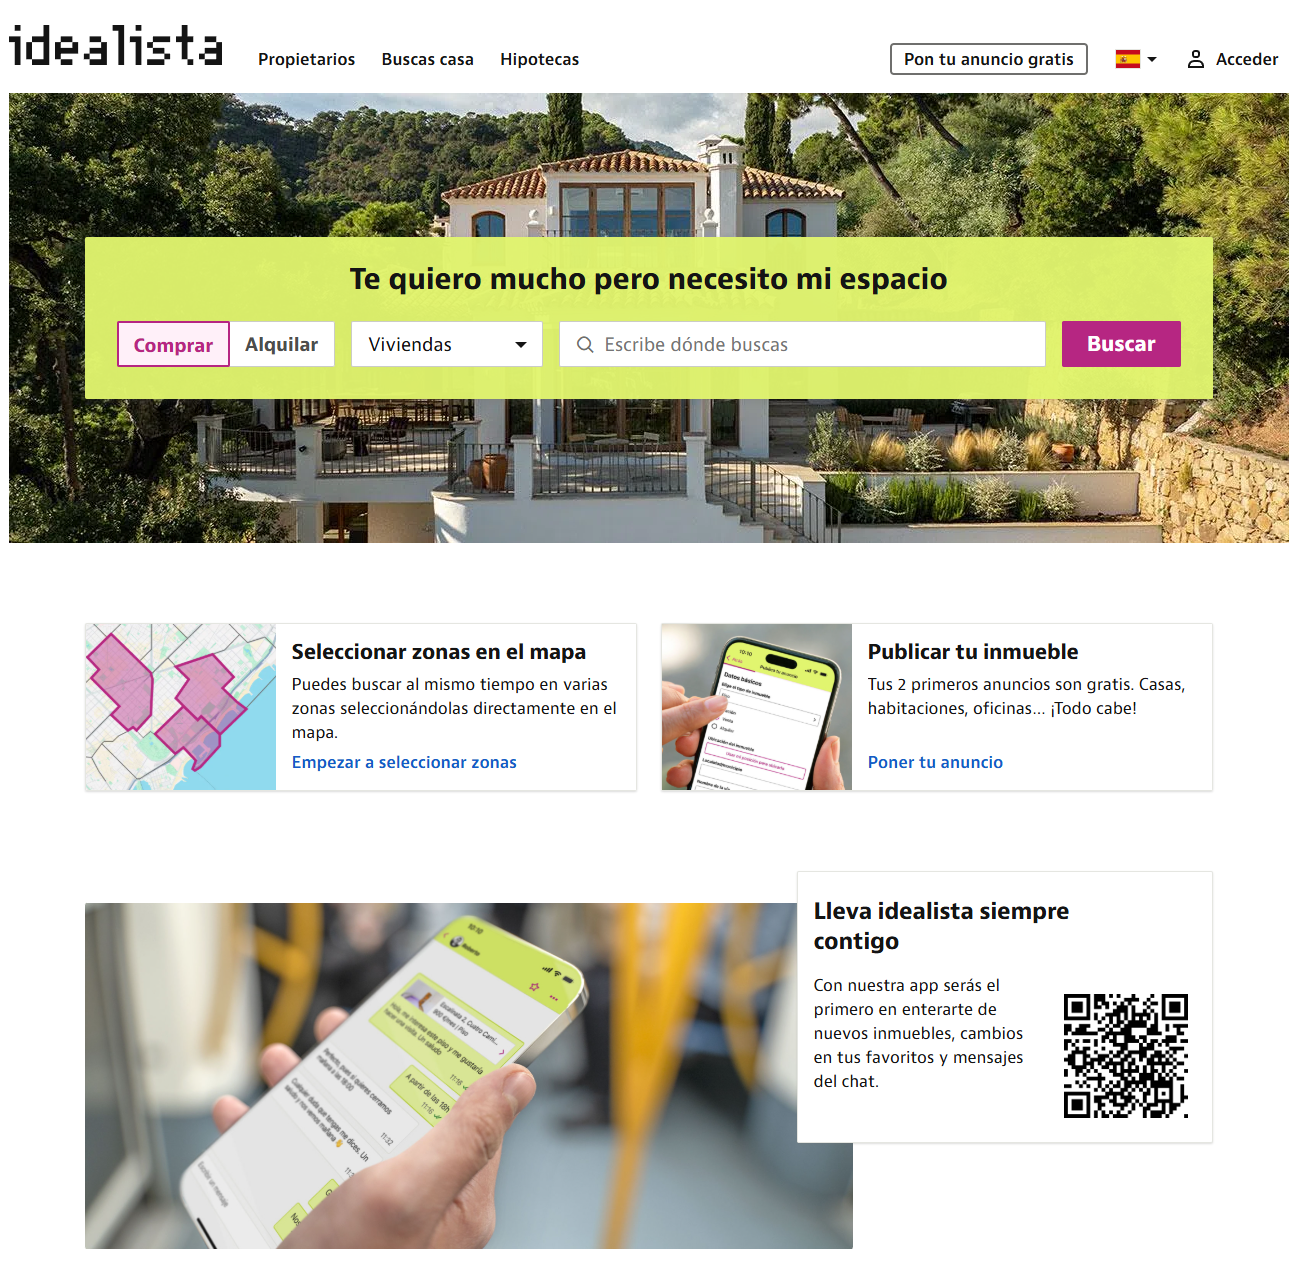
\includegraphics[width=\linewidth,height=7.8cm,keepaspectratio]{Introduccion/img/Idealista.png}
        \caption{Búsqueda en Idealista}
        \label{subfig:idealista}
    \end{subfigure}
    \hfill
    \begin{subfigure}[b]{0.49\textwidth}
        \centering
        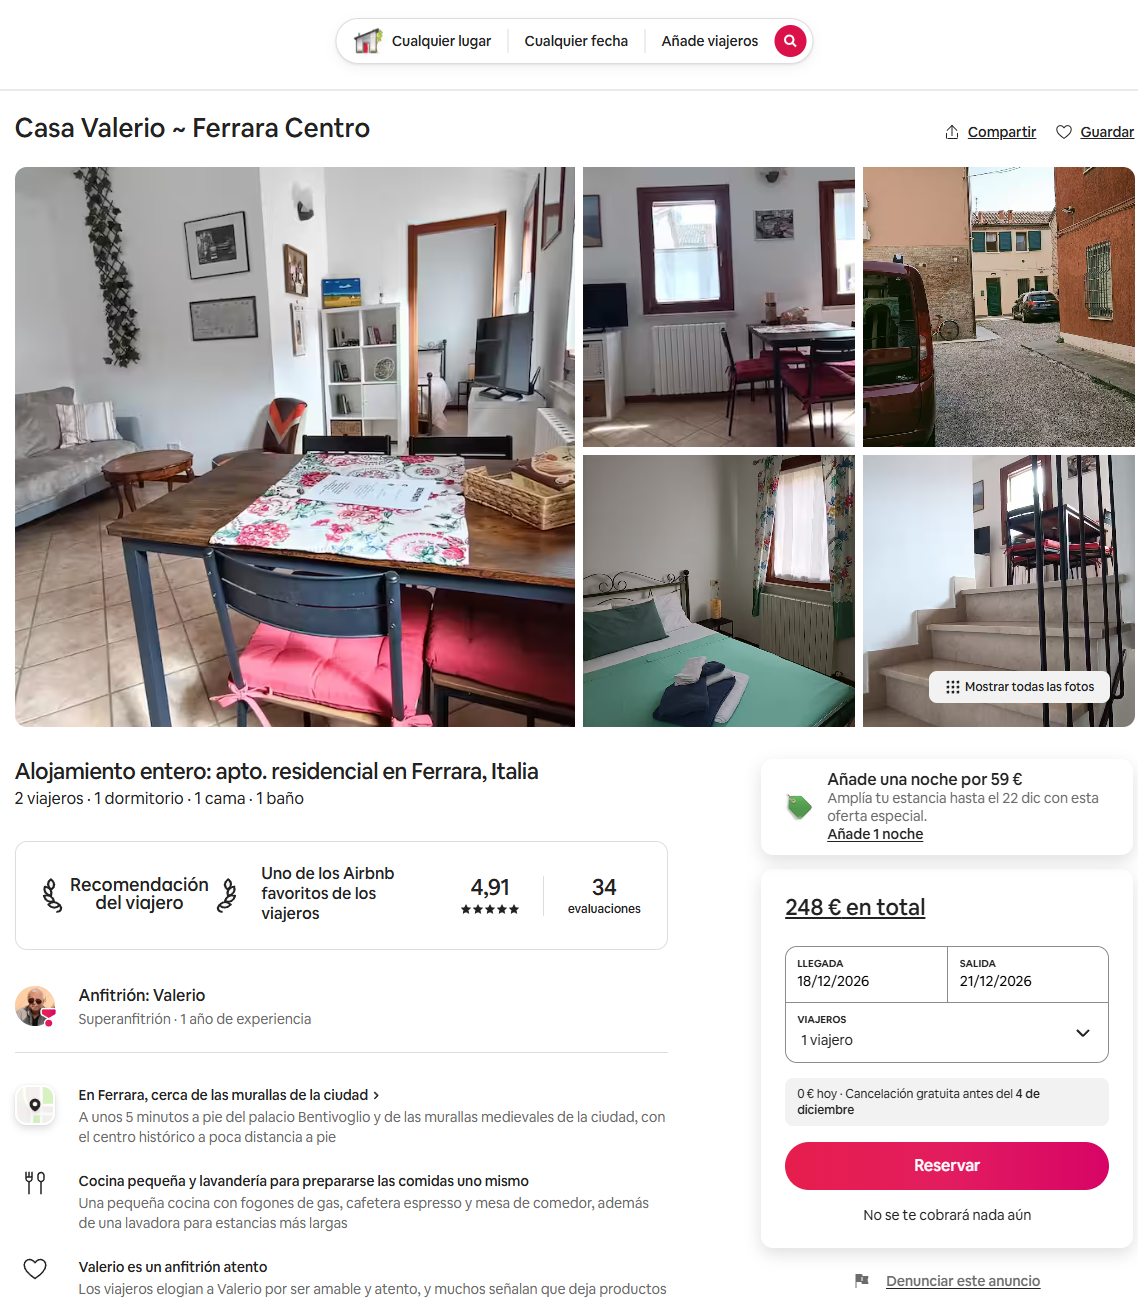
\includegraphics[width=\linewidth,height=7.8cm,keepaspectratio]{Introduccion/img/Airbnb.png}
        \caption{Detalles y reserva en Airbnb}
        \label{subfig:airbnb}
    \end{subfigure}
    
    \vspace{0.4cm}
    
    \begin{subfigure}[b]{0.49\textwidth}
        \centering
        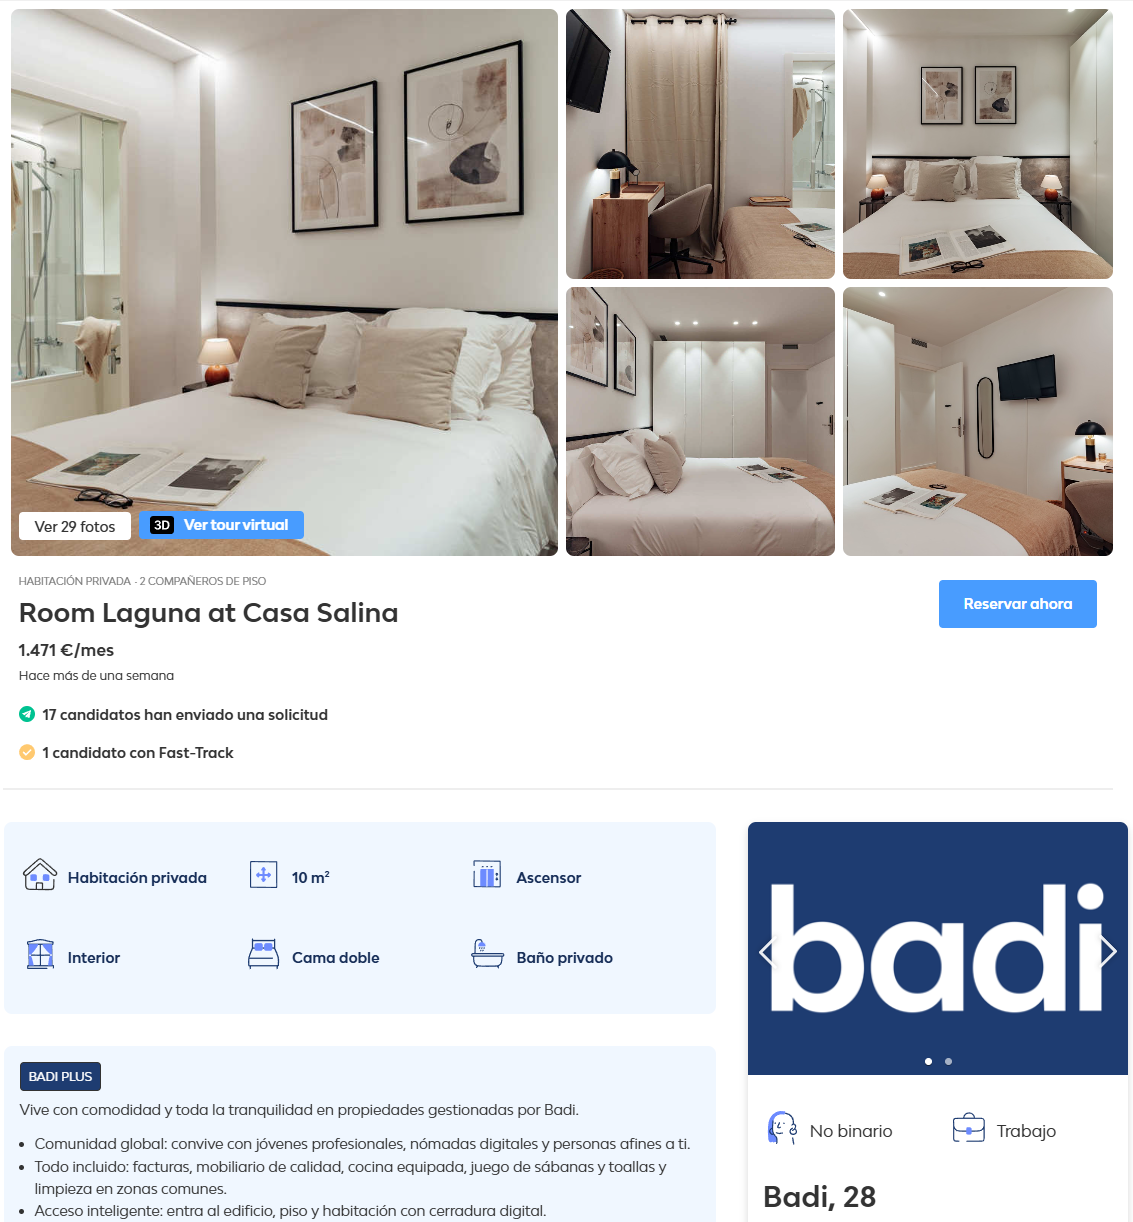
\includegraphics[width=\linewidth,height=7.8cm,keepaspectratio]{Introduccion/img/Badi.png}
        \caption{Habitaciones y perfiles en Badi}
        \label{subfig:badi}
    \end{subfigure}
    \hfill
    \begin{subfigure}[b]{0.49\textwidth}
        \centering
        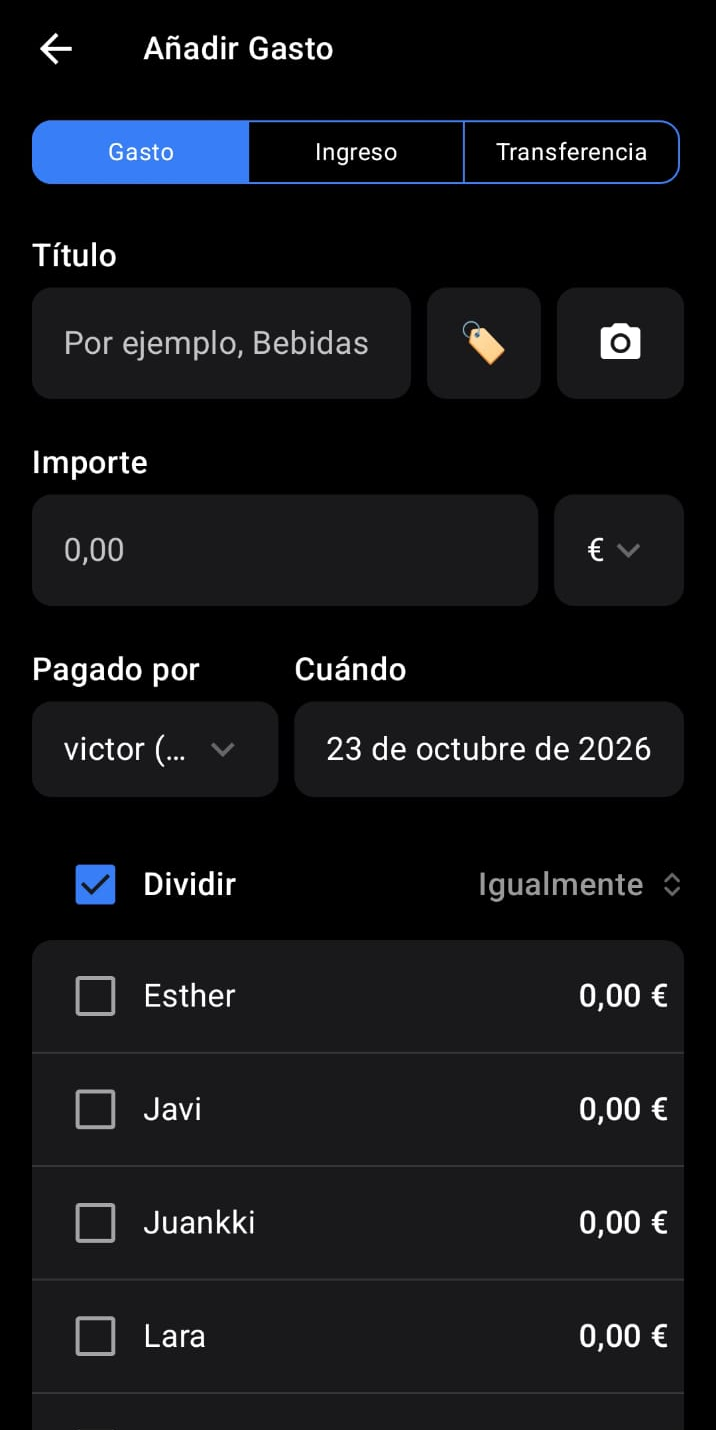
\includegraphics[width=\linewidth,height=7.8cm,keepaspectratio]{Introduccion/img/Tricount.png}
        \caption{Reparto de gastos en Tricount}
        \label{subfig:tricount}
    \end{subfigure}
    \caption{Interfaces de las principales soluciones analizadas en el mercado}
    \label{fig:apps_similares}
\end{figure}

    El ecosistema digital actual fragmenta la experiencia del inquilino en aplicaciones independientes sin conexión entre sí. Los usuarios buscan habitación en una web, firman el contrato en persona, anotan los gastos en una aplicación externa y discuten la limpieza por mensajería. Colivi unifica estas fases bajo una sola plataforma web y móvil, incorporando además un asistente basado en MCP para interactuar con los datos del hogar.

\begin{table}[htbp]
    \centering
    \caption{Comparativa de características entre plataformas analizadas y Colivi}
    \label{tab:comparativa_apps}
    \vspace{0.2cm}
    \resizebox{\textwidth}{!}{%
    \begin{tabular}{|l|c|c|c|c|c|c|}
        \hline
        \textbf{Plataforma} & \textbf{\begin{tabular}[c]{@{}c@{}}Catálogo y\\ Búsqueda\end{tabular}} & \textbf{\begin{tabular}[c]{@{}c@{}}Reserva y Fianza\\ Integrada\end{tabular}} & \textbf{\begin{tabular}[c]{@{}c@{}}Reparto de\\ Gastos Comunes\end{tabular}} & \textbf{\begin{tabular}[c]{@{}c@{}}Gamificación\\ de Tareas\end{tabular}} & \textbf{\begin{tabular}[c]{@{}c@{}}Asistente\\ IA (MCP)\end{tabular}} & \textbf{\begin{tabular}[c]{@{}c@{}}Enfoque\\ Coliving\end{tabular}} \\ \hline
        Idealista & Sí & No & No & No & No & No \\ \hline
        Airbnb & Sí & Sí & No & No & No & No \\ \hline
        Badi & Sí & No & No & No & No & Sí \\ \hline
        Tricount & No & No & Sí & No & No & No \\ \hline
        \textbf{Colivi (Propuesta)} & \textbf{Sí} & \textbf{Sí} & \textbf{Sí} & \textbf{Sí} & \textbf{Sí} & \textbf{Sí} \\ \hline
    \end{tabular}%
    }
\end{table}

    Las columnas de la tabla comparativa evalúan las siguientes capacidades técnicas y de dominio:

\begin{itemize}
    \item \textbf{Catálogo y Búsqueda}: motor público de localización con filtros espaciales, rangos de precio y comodidades del inmueble. Portales como Idealista, Airbnb y Badi satisfacen este criterio, mientras que utilidades contables como Tricount o Flatastic carecen de catálogo por definición.
    \item \textbf{Reserva y Fianza Integrada}: capacidad para formalizar acuerdos de estancia y retener o transferir depósitos de garantía mediante pasarelas auditables dentro del propio sistema. Solo Airbnb soporta este flujo en el mercado actual, pues Idealista y Badi delegan las transacciones económicas a pactos privados fuera de la plataforma.
    \item \textbf{Reparto de Gastos Comunes}: presencia de un motor de liquidación para prorratear facturas, calcular saldos individuales y registrar transferencias compensatorias. Supone el núcleo de Tricount, pero los portales de alquiler lo omiten en su totalidad.
    \item \textbf{Gamificación de Tareas}: mecanismos de rotación periódica del trabajo doméstico apoyados en asignaciones equitativas y tablas de clasificación. Únicamente Flatastic aproxima este concepto, aunque con métricas básicas sin trazabilidad inmutable del hogar.
    \item \textbf{Asistente IA (MCP)}: integración de un agente conversacional capaz de ejecutar herramientas sobre la base de datos del piso mediante el protocolo \emph{Model Context Protocol}. Ningún competidor del mercado incorpora agentes con acceso contextual al estado de tareas o finanzas de la vivienda.
    \item \textbf{Enfoque Coliving}: diseño centrado en el arrendamiento por habitaciones con zonas comunes y convivencia comunitaria entre estudiantes o jóvenes profesionales. Badi y Flatastic comparten esta orientación, diferenciándose de modelos turísticos o residenciales familiares.
\end{itemize}

Determinadas características exigen matices técnicos. Badi, por ejemplo, gestiona un cobro inicial para formalizar la reserva, pero no asume la custodia ni la restitución de la fianza durante la vigencia del contrato de arrendamiento. De igual forma, las opciones de atención automatizada en portales como Airbnb se limitan a centros de ayuda estáticos con preguntas frecuentes, sin conectividad hacia un servidor de contexto capaz de inspeccionar los registros internos del alojamiento.

\section{Contenido de la memoria}
\label{Contenido de la memoria}

    La presente memoria se encuentra estructurada en diversos capítulos que recogen, de manera sistemática y progresiva, las fases de análisis, diseño, desarrollo y validación de Colivi, una plataforma web y móvil asistida por inteligencia artificial orientada a la gestión integral del alquiler en régimen de coliving y a la convivencia entre residentes. A continuación, se resume de forma sucinta el propósito y contenido de cada una de las partes que integran este trabajo:

- Introducción: se contextualiza la creciente demanda del modelo residencial de coliving entre estudiantes y jóvenes profesionales, exponiendo las problemáticas actuales asociadas a la dispersión de herramientas digitales durante la búsqueda de piso y la convivencia diaria.

- Justificación: se detallan las razones técnicas y sociales que motivan la elección de esta propuesta, destacando la oportunidad de resolver la fragmentación operativa del alquiler compartido unificando el ciclo completo en una sola solución con soporte inteligente.

- Objetivos: se formula el objetivo general del proyecto y se desglosan los objetivos específicos, delimitando el alcance funcional de la plataforma tanto en la vertiente web como en su empaquetado móvil.

- Planificación: se describe la organización temporal del desarrollo a partir de un ciclo de vida clásico de ingeniería del software, exponiendo las fases del proyecto, el cronograma de trabajo planificado en 300 horas lectivas y la trazabilidad de las dependencias lógicas.

- Aplicaciones similares: se ofrece un análisis comparativo frente a soluciones existentes en el mercado (portales de búsqueda inmobiliaria, plataformas de alojamiento temporal y utilidades de reparto de gastos), delimitando los criterios funcionales que diferencian y fundamentan la propuesta de Colivi.

- Herramientas y tecnologías: se justifican las decisiones metodológicas y la selección del stack tecnológico empleado, profundizando en el backend con Java 21 y Spring Boot 3, el frontend reactivo con React, TypeScript y Tailwind CSS, la persistencia relacional con PostgreSQL, la integración del protocolo Model Context Protocol (MCP) con Spring AI y Groq, y la adaptación móvil mediante Capacitor.
 
- Análisis y diseño del sistema: se documentan los diferentes roles de usuario, el catálogo riguroso de requisitos funcionales y no funcionales, los diagramas de casos de uso, el modelo entidad-relación de la base de datos y la arquitectura distribuida del sistema desacoplada bajo principios SOLID.

- Implementación del sistema: se expone detalladamente el desarrollo técnico modular de la plataforma, abordando el control de acceso sin estado con JWT, el catálogo con mapas interactivos, el flujo de reservas con fianza integrada y control de concurrencia, los módulos de convivencia del hogar (gastos compartidos, tareas domésticas con asignación rotativa y mensajería interna) y el microservicio MCP que da soporte al asistente conversacional.

- Adaptabilidad móvil y despliegue: se describe la optimización ergonómica de la interfaz de usuario para dispositivos móviles, el empaquetado del aplicativo para Android y la configuración de la infraestructura mediante contenedores Docker y servicios cloud en Microsoft Azure con automatización CI/CD.

- Plan de pruebas y aseguramiento de la calidad: se detalla la estrategia de verificación adoptada, cubriendo las pruebas unitarias y de integración de la lógica de negocio, las comprobaciones de los endpoints seguros y el análisis de incidencias técnicas resueltas durante el desarrollo.

- Estudio de costes: se desglosa el presupuesto global estimado para la ejecución del proyecto, cuantificando los costes derivados del esfuerzo humano (horas de ingeniería), la infraestructura cloud, las herramientas de desarrollo y los recursos materiales requeridos.

- Conclusiones y líneas futuras: se sintetizan las metas alcanzadas y el grado de cumplimiento de los objetivos planteados, proponiendo posibles vías de evolución técnica para extender las capacidades operativas y de inteligencia del sistema.

- Bibliografía: se recopilan formalmente todas las referencias bibliográficas, documentación técnica oficial, especificaciones de protocolos, estándares y fuentes académicas consultadas a lo largo de la investigación y construcción de la memoria.
